\documentclass[12pt,letterpaper,twoside]{article}
\usepackage{amsmath,amssymb,amsfonts}
\usepackage{graphicx}
\usepackage{tikz}
\usepackage{pgfplots}
\pgfplotsset{compat=1.17}
\usepackage{xcolor}
\usepackage{hyperref}
\usepackage{cleveref}
\usepackage{booktabs}
\usepackage{caption}
\usepackage{subcaption}
\usepackage{wrapfig}
\usepackage{nicefrac}
\usepackage{minted}
\usepackage{geometry}
\geometry{margin=1in, top=0.75in, bottom=0.75in}

% Colors for symplectic attention visualization
\definecolor{symplectblue}{RGB}{31, 119, 180}
\definecolor{symplectred}{RGB}{214, 39, 40}
\definecolor{symplectgreen}{RGB}{44, 160, 44}
\definecolor{symplectpurple}{RGB}{148, 103, 189}
\definecolor{symplectorange}{RGB}{255, 127, 14}
\definecolor{symplectteal}{RGB}{44, 174, 175}
\definecolor{symplectyellow}{RGB}{188, 189, 34}

% TikZ libraries
\usetikzlibrary{decorations.pathmorphing,shapes.geometric,calc,positioning,arrows.meta,patterns}

% Title and Author
\title{\textbf{Symplectic Attention: Constant-Memory Sequence Modeling via Geodesic Flow}}

\author{Joaquin Stürtz}

\date{January 24, 2026}

% Header
\pagestyle{myheadings}
\markright{Symplectic Attention: Geodesic Flow}
\lhead{Manifold Learning Research}
\rhead{\thepage}

% Theorem-like environments
\newtheorem{definition}{Definition}[section]
\newtheorem{theorem}{Theorem}[section]
\newtheorem{Lemma}{Lemma}[section]
\newtheorem{example}{Example}[section]
\newtheorem{remarque}{Remark}[section]
\newtheorem{prop}{Proposition}[section]
\newtheorem{corol}{Corollary}[section]

% Macros for frequently used notation
\newcommand{\M}{\mathcal{M}}
\newcommand{\R}{\mathbb{R}}
\newcommand{\T}{\mathbb{T}}
\newcommand{\Sph}{\mathbb{S}}
\newcommand{\diff}{\mathrm{d}}
\DeclareMathOperator{\Tr}{Tr}
\DeclareMathOperator{\diag}{diag}
\DeclareMathOperator{\sech}{sech}

\begin{document}

\maketitle
\thispagestyle{empty}

\vspace{0.5cm}

\begin{abstract}
Attention computes non-local interactions over a growing memory of keys and values, incurring quadratic time and linear memory with sequence length. We claim that this explicit global lookup is not necessary if the model's recurrence obeys a physically grounded dynamical law. \textbf{Symplectic Attention} replaces pairwise token interactions with \textbf{local geodesic flow} on a learned manifold: the model carries its causal history in a compact phase state $(x_t, v_t)$, and "attends" by evolving along learned curvature with structure-preserving integrators. A learned friction gate provides selective irreversibility for state rewriting, while a curvature-informed time gate shrinks steps in complex regions. The result is constant-memory inference with linear time, verified by a reference implementation based on multi-head manifolds, toroidal topology, and symplectic integration.
\end{abstract}

\vspace{0.5cm}
\hrule
\vspace{0.5cm}

\tableofcontents
\newpage

\section{Motivation: From Global Lookup to Local Flow}

The Transformer architecture has revolutionized deep learning, but its attention mechanism carries fundamental computational costs. Symplectic Attention offers a physically grounded alternative that replaces quadratic global lookups with linear local flow.

\subsection{The Cost of ``Action at a Distance''}

Transformers maintain a full history of Key-Value pairs $(K, V)$ and, to produce the next output, query this entire memory:

\begin{definition}[Transformer Attention]
\[
\text{Attention}(Q, K, V) = \softmax\left(\frac{QK^\top}{\sqrt{d}}\right) V.
\]
\end{definition}

This non-local operation has serious scaling limitations:

\begin{prop}[Attention Complexity]
\begin{enumerate}
\item \textbf{Time complexity}: $O(N^2)$ per layer, where $N$ is sequence length.
\item \textbf{Memory complexity}: $O(N^2)$ for storing attention matrices during training.
\item \textbf{Inference memory}: Grows linearly with context ($O(N)$ KV cache).
\end{enumerate}
\end{prop}

More fundamentally, this assumes relevant information must be explicitly retrieved from a static cache rather than propagated causally through time.

\begin{remarque}[Conceptual Limitation]
The attention mechanism treats all past tokens equally at each step, computing $O(N^2)$ interactions regardless of whether information is relevant. This is unlike physical systems, where influence propagates locally through fields.
\end{remarque}

\begin{figure}[htbp]
\centering
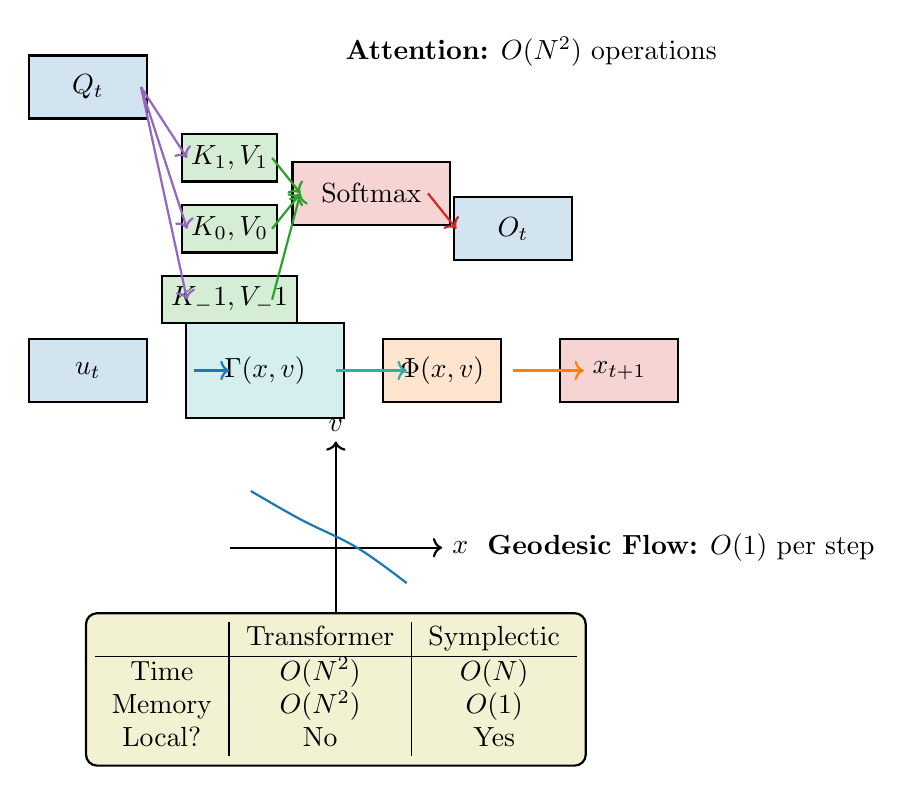
\begin{tikzpicture}[scale=0.9]
    % Transformer attention diagram
    \node[draw, rectangle, fill=symplectblue!20, thick, minimum width=1.5cm, minimum height=0.8cm] at (0, 2) {$Q_t$};
    
    \foreach \y in {-1,0,1} {
        \node[draw, rectangle, fill=symplectgreen!20, thick, minimum width=1.2cm, minimum height=0.6cm] at (2, \y) {$K_\y, V_\y$};
        \draw[->, thick, symplectpurple] (0.75, 2) -- (1.4, \y);
    }
    
    \node[draw, rectangle, fill=symplectred!20, thick, minimum width=2cm, minimum height=0.8cm] at (4, 0.5) {Softmax};
    
    \node[draw, rectangle, fill=symplectblue!20, thick, minimum width=1.5cm, minimum height=0.8cm] at (6, 0) {$O_t$};
    
    \draw[->, thick, symplectgreen] (2.6, -1) -- (3, 0.5);
    \draw[->, thick, symplectgreen] (2.6, 0) -- (3, 0.5);
    \draw[->, thick, symplectgreen] (2.6, 1) -- (3, 0.5);
    \draw[->, thick, symplectred] (4.8, 0.5) -- (5.2, 0);
    
    % Label
    \node[right] at (3.5, 2.5) {\textbf{Attention:} $O(N^2)$ operations};
    
    % Symplectic alternative
    \begin{scope}[shift={(0, -4)}]
        \node[draw, rectangle, fill=symplectblue!20, thick, minimum width=1.5cm, minimum height=0.8cm] at (0, 2) {$u_t$};
        
        \node[draw, rectangle, fill=symplectteal!20, thick, minimum width=2cm, minimum height=1.2cm] at (2.5, 2) {$\Gamma(x,v)$};
        
        \node[draw, rectangle, fill=symplectorange!20, thick, minimum width=1.5cm, minimum height=0.8cm] at (5, 2) {$\Phi(x,v)$};
        
        \node[draw, rectangle, fill=symplectred!20, thick, minimum width=1.5cm, minimum height=0.8cm] at (7.5, 2) {$x_{t+1}$};
        
        \draw[->, thick, symplectblue] (1.5, 2) -- (2, 2);
        \draw[->, thick, symplectteal] (3.5, 2) -- (4.5, 2);
        \draw[->, thick, symplectorange] (6, 2) -- (7, 2);
        
        % Phase space inset
        \begin{scope}[shift={(3.5, -0.5)}]
            \draw[->, thick] (-1.5, 0) -- (1.5, 0) node[right] {$x$};
            \draw[->, thick] (0, -1.5) -- (0, 1.5) node[above] {$v$};
            
            \draw[symplectblue, thick] 
                plot[smooth,tension=0.6] coordinates {
                    (-1.2, 0.8) (-0.5, 0.4) (0.3, 0) (1.0, -0.5)
                };
        \end{scope}
        
        \node[right] at (5.5, -0.5) {\textbf{Geodesic Flow:} $O(1)$ per step};
    \end{scope}
    
    % Complexity comparison
    \node[draw, rectangle, rounded corners, fill=symplectyellow!20, thick] at (3.5, -6.5) {
        \begin{tabular}{c|c|c}
            & Transformer & Symplectic \\ \hline
            Time & $O(N^2)$ & $O(N)$ \\
            Memory & $O(N^2)$ & $O(1)$ \\
            Local? & No & Yes
        \end{tabular}
    };
\end{tikzpicture}
\caption{Comparison of Transformer attention (top) and Symplectic Attention (bottom). While Transformers query all past tokens globally, Symplectic Attention propagates information through local geodesic flow on a learned manifold.}
\label{fig:attention-comparison}
\end{figure}

\subsection{The Physical Alternative}

In physics, a particle does not query distant points; it moves under local fields. The "memory" of past interactions is encoded in geometry (metric and connection), and the trajectory reveals which past impulses matter.

\begin{prop}[Physical Philosophy]
\begin{enumerate}
\item \textbf{Locality}: Interactions occur only at the particle's current position.
\item \textbf{Geometry encodes history}: The metric and connection encode how past forces shape present motion.
\item \textbf{Propagation through flow}: Information propagates continuously through the dynamical system.
\end{enumerate}
\end{prop}

Symplectic Attention reformulates sequence modeling so that "attention" arises from \textbf{geodesic deviation}: the state flows along learned curvature that locally encodes how past tokens shape present motion.

\begin{remarque}[Key Insight]
Instead of explicitly storing and retrieving all past information, the model carries a compact phase state $(x_t, v_t)$ that implicitly encodes causal history through momentum and winding on a compact manifold.
\end{remarque}

\section{Continuous-Time Formalism}

We augment Hamiltonian dynamics with learned curvature and selective dissipation, creating a continuous-time foundation for Symplectic Attention.

\begin{definition}[Symplectic Attention Dynamics]
The continuous-time evolution is:
\[
\dot{x} = v, \quad \dot{v} = F_\theta(u_t) - \Gamma_\theta(x, v) - \mu_\theta(x, u_t) \odot v,
\]
where:
\begin{itemize}
\item $F_\theta(u_t)$ maps tokens to force impulses,
\item $\Gamma_\theta(x, v)$ is a learned Christoffel-like interaction encoding geometric coupling,
\item $\mu_\theta(x, u_t) \geq 0$ is a friction "clutch" that switches between conservative memory and dissipative updating,
\item $\odot$ denotes element-wise multiplication.
\end{itemize}
\end{definition}

This single equation captures the full dynamics of Symplectic Attention.

\subsection{Symplectic Attention as Geodesic Flow}

Instead of $O(N^2)$ pairwise weighting, past tokens influence the present through the shape of the trajectory:

\begin{prop}[Attention via Geometry]
\begin{enumerate}
\item \textbf{Phase state encoding}: The instantaneous phase state $(x_t, v_t)$ encodes causal history as momentum and winding on a compact manifold.
\item \textbf{Geometric attention}: "Attending" is realized by local curvature steering—the geometry determines which past influences matter at each moment.
\item \textbf{Physical forgetting}: Dissipation ($\mu > 0$) opens the clutch to overwrite state during transitions, implementing forgetting physically rather than numerically.
\end{enumerate}
\end{prop}

This is fundamentally different from attention:

\begin{remarque}[Conceptual Difference]
\begin{itemize}
\item \textbf{Attention}: Explicitly compute weighted sum over all past tokens.
\item \textbf{Symplectic Attention}: Let information flow naturally through geometry; the trajectory encodes which past influences matter.
\end{itemize}
\end{remarque}

\begin{figure}[htbp]
\centering
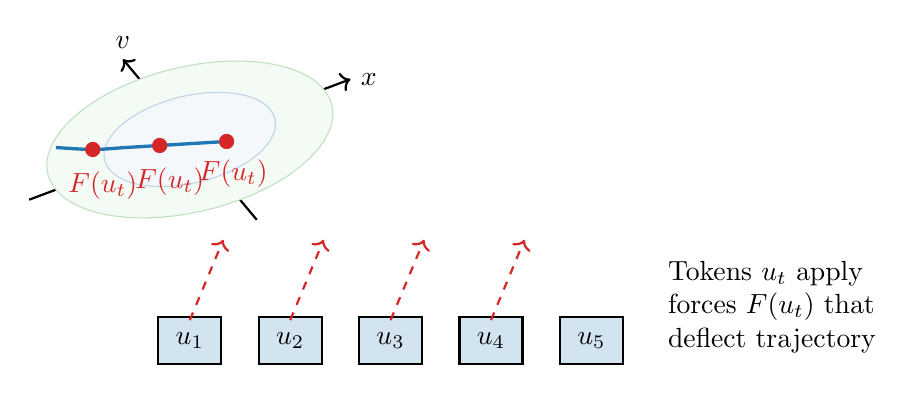
\begin{tikzpicture}[scale=0.85]
    % Phase space trajectory
    \begin{scope}[x={(0.8cm,0.3cm)},y={(-0.5cm,0.6cm)},z={(0cm,1cm)}]
        % Phase space container
        \draw[->, thick] (-3, 0, 0) -- (3, 0, 0) node[right] {$x$};
        \draw[->, thick] (0, -2, 0) -- (0, 2, 0) node[above] {$v$};
        
        % Energy contours
        \draw[symplectgreen!30, fill=symplectgreen!5] 
            ellipse (2.5 and 1.5);
        \draw[symplectblue!30, fill=symplectblue!5] 
            ellipse (1.5 and 0.9);
            
        % Trajectory with impulse events
        \draw[symplectblue, very thick] 
            plot[smooth,tension=0.5] coordinates {
                (-2, 0.8, 0) (-1.5, 0.5, 0) (-1, 0.3, 0) 
                (-0.5, 0.1, 0) (0, -0.1, 0) (0.5, -0.3, 0)
            };
            
        % Impulse markers
        \filldraw[symplectred] (-1.5, 0.5, 0) circle (3pt);
        \filldraw[symplectred] (-0.5, 0.1, 0) circle (3pt);
        \filldraw[symplectred] (0.5, -0.3, 0) circle (3pt);
        
        % Labels
        \node[symplectred, below] at (-1.5, 0.2, 0) {$F(u_t)$};
        \node[symplectred, below] at (-0.5, -0.2, 0) {$F(u_t)$};
        \node[symplectred, below] at (0.5, -0.5, 0) {$F(u_t)$};
    \end{scope}
    
    % Token sequence
    \node[draw, rectangle, fill=symplectblue!20, thick, minimum width=0.8cm, minimum height=0.6cm] at (0, -3) {$u_1$};
    \node[draw, rectangle, fill=symplectblue!20, thick, minimum width=0.8cm, minimum height=0.6cm] at (1.5, -3) {$u_2$};
    \node[draw, rectangle, fill=symplectblue!20, thick, minimum width=0.8cm, minimum height=0.6cm] at (3, -3) {$u_3$};
    \node[draw, rectangle, fill=symplectblue!20, thick, minimum width=0.8cm, minimum height=0.6cm] at (4.5, -3) {$u_4$};
    \node[draw, rectangle, fill=symplectblue!20, thick, minimum width=0.8cm, minimum height=0.6cm] at (6, -3) {$u_5$};
    
    % Arrows showing token influence
    \foreach \x/\tx in {0/1, 1.5/2, 3/3, 4.5/4} {
        \draw[->, thick, symplectred, dashed] (\x, -2.7) -- (\x + 0.5, -1.5);
    }
    
    % Explanation
    \node[right] at (7, -2) {Tokens $u_t$ apply};
    \node[right] at (7, -2.5) {forces $F(u_t)$ that};
    \node[right] at (7, -3) {deflect trajectory};
\end{tikzpicture}
caption{Symplectic Attention as geodesic flow. Tokens $u_t$ apply forces $F(u_t)$ that deflect the phase-space trajectory. The geometry $\Gamma(x,v)$ determines how past influences propagate forward.}
\label{fig:geodesic-flow}
\end{figure}

\subsection{Multi-Head Manifolds}

Analogous to multi-head attention, we factor the latent into $H$ heads, each with its own geometry and gates:

\begin{definition}[Multi-Head Architecture]
The phase state is decomposed as:
\[
(x, v) = \bigoplus_{h=1}^{H} (x^{(h)}, v^{(h)}),
\]
where each head $(x^{(h)}, v^{(h)})$ maintains:
\begin{itemize}
\item Its own geometry $\Gamma_\theta^{(h)}(x^{(h)}, v^{(h)})$,
\item Its own friction gate $\mu_\theta^{(h)}(x^{(h)}, u_t)$,
\item Its own time gate $g^{(h)}(x^{(h)})$.
\end{itemize}
\end{definition}

Heads evolve in parallel, then are mixed back into the shared state. This yields diverse relational channels without constructing global attention matrices.

\begin{prop}[Head Diversity]
Each head can specialize for different types of relationships:
\begin{enumerate}
\item Different curvature patterns for different temporal structures.
\item Different gating thresholds for different update frequencies.
\end{enumerate}
\end{prop}

\begin{remarque}[Parallelism Benefit]
Multi-head structure is naturally parallel: all heads can be updated simultaneously, then combined through learned linear mixing.
\end{remarque}

\begin{figure}[htbp]
\centering
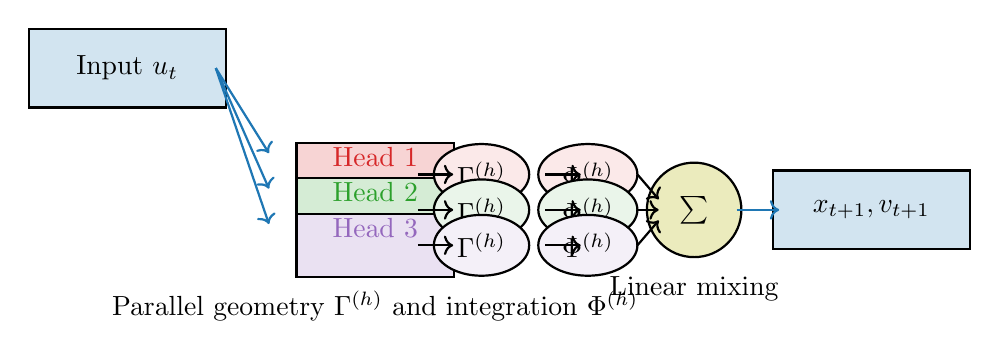
\begin{tikzpicture}[scale=0.9]
    % Multi-head architecture
    \node[draw, rectangle, fill=symplectblue!20, thick, minimum width=2.5cm, minimum height=1cm] at (0, 2) {Input $u_t$};
    
    % Heads
    \foreach \y/\col/\lab in {0.5/symplectred/Head 1, 0/symplectgreen/Head 2, -0.5/symplectpurple/Head 3} {
        \node[draw, rectangle, fill=\col!20, thick, minimum width=2cm, minimum height=0.8cm] at (3.5, \y) {};
        \node[\col] at (3.5, \y + 0.25) {\lab};
    }
    
    % Connections
    \draw[->, thick, symplectblue] (1.25, 2) -- (2, 0.8);
    \draw[->, thick, symplectblue] (1.25, 2) -- (2, 0.3);
    \draw[->, thick, symplectblue] (1.25, 2) -- (2, -0.2);
    
    % Geometry and integration within each head
    \foreach \y/\col in {0.5/symplectred, 0/symplectgreen, -0.5/symplectpurple} {
        \node[draw, ellipse, fill=\col!10, thick, minimum width=0.8cm, minimum height=0.6cm] at (5, \y) {$\Gamma^{(h)}$};
        \node[draw, ellipse, fill=\col!10, thick, minimum width=0.8cm, minimum height=0.6cm] at (6.5, \y) {$\Phi^{(h)}$};
        \draw[->, thick] (4.1, \y) -- (4.6, \y);
        \draw[->, thick] (5.9, \y) -- (6.4, \y);
    }
    
    % Mixing
    \node[draw, circle, fill=symplectyellow!30, thick, minimum size=1.2cm] at (8, 0) {$\sum$};
    
    \foreach \y in {0.5, 0, -0.5} {
        \draw[->, thick] (7.2, \y) -- (7.5, \y * 0.3);
    }
    
    % Output
    \node[draw, rectangle, fill=symplectblue!20, thick, minimum width=2.5cm, minimum height=1cm] at (10.5, 0) {$x_{t+1}, v_{t+1}$};
    
    \draw[->, thick, symplectblue] (8.6, 0) -- (9.2, 0);
    
    % Labels
    \node[below] at (3.5, -1) {Parallel geometry $\Gamma^{(h)}$ and integration $\Phi^{(h)}$};
    \node[below] at (8, -0.8) {Linear mixing};
\end{tikzpicture}
caption{Multi-head architecture for Symplectic Attention. Each head maintains independent geometry and gates, evolves in parallel, then is mixed back into the global state.}
\label{fig:multi-head-symplectic}
\end{figure}

\subsection{Dynamic Time and Selective Irreversibility}

Two learned gates provide additional control:

\begin{definition}[Control Gates]
\begin{enumerate}
\item \textbf{Time gate}: $g(x) \in (0, 1]$ scales the effective step size in "hard" regions (high curvature):
\[
\Delta t_{\text{eff}} = g(x) \cdot \Delta t.
\]

\item \textbf{Friction gate}: $\mu(x, u) \geq 0$ controls when to dissipate momentum and rewrite the state.
\end{enumerate}
\end{definition}

Together they implement stable, controllable computation over long horizons:

\begin{prop}[Gate Functions]
\begin{itemize}
\item \textbf{Time contraction} ($g < 1$): Smaller steps in high-curvature regions prevent numerical instability and aliasing.
\item \textbf{Dissipation} ($\mu > 0$): Momentum damping enables state rewriting at semantic transitions.
\end{itemize}
\end{prop}

\subsection{Symplectic Stability}

The $\mu = 0$ regime exhibits fundamental stability properties:

\begin{prop}[Symplectic Properties]
When $\mu = 0$:
\begin{enumerate}
\item The update is \textbf{symplectic}: phase-space volume is preserved.
\item \textbf{Gradients neither vanish nor explode}: Hamiltonian systems have bounded sensitivity to initial conditions.
\item \textbf{Long-term stability}: Liouville's theorem ensures information about initial conditions is preserved.
\end{enumerate}
\end{prop}

Forgetting arises physically through $\mu > 0$, not numerically through unstable mappings. This is a fundamental difference from RNNs, where vanishing gradients limit memory.

\begin{remarque}[Physical Forgetting]
In Symplectic Attention, "forgetting" is not a numerical failure but a physical process (dissipation) that can be learned and controlled. This provides principled control over the memory/update trade-off.
\end{remarque}

\section{Discretization: Symplectic Attention Step}

We discretize the continuous dynamics using structure-preserving integrators.

\begin{definition}[Symplectic Attention Leapfrog Step]
Let $\Delta t$ be the base step, $g(x) \in (0, 1]$ the time gate, $\Delta t_{\text{eff}} = g(x) \Delta t$, and $h = \frac{1}{2} \Delta t_{\text{eff}}$. A single head applies:

\begin{enumerate}
\item \textbf{Kick} (half-step, implicit damping):
\[
v_{n+\frac{1}{2}} = \frac{v_n + h \cdot [F_\theta(u_n) - \Gamma_\theta(x_n, v_n)]}{1 + h \cdot \mu_\theta(x_n, u_n)}.
\]

\item \textbf{Drift} (full-step position with topology):
\[
x_{n+1} = \operatorname{wrap}\!\left(x_n + \Delta t_{\text{eff}} \cdot v_{n+\frac{1}{2}}\right).
\]

\item \textbf{Kick} (half-step at new position):
\[
v_{n+1} = \frac{v_{n+\frac{1}{2}} + h \cdot [F_\theta(u_n) - \Gamma_\theta(x_{n+1}, v_{n+\frac{1}{2}})]}{1 + h \cdot \mu_\theta(x_{n+1}, u_n)}.
\]
\end{enumerate}
\end{definition}

The implicit friction form $\frac{v}{1 + h\mu}$ ensures stability even for large $\mu$.

\begin{prop}[Step Properties]
\begin{enumerate}
\item \textbf{Symplectomorphism} ($\mu = 0$): The map preserves the symplectic 2-form $\omega = dx \wedge dv$.
\item \textbf{Controlled dissipation} ($\mu > 0$): Phase-space volume contracts at rate $\mu$.
\item \textbf{Topology preservation}: $\operatorname{wrap}(\cdot)$ maintains coordinates on the manifold.
\end{enumerate}
\end{prop}

Heads evolve in parallel; their states are concatenated and linearly mixed back into $(x, v)$. The scheme generalizes to other symplectic integrators (Yoshida, Forest-Ruth, Omelyan) and high-order explicit schemes (Heun/RK4/RK45) when conservation needs trade-off against local accuracy.

\begin{remarque}[Integrator Choice]
For smooth dynamics, higher-order symplectic methods reduce integration error. For non-smooth dynamics, RK methods provide more robustness at the cost of symplectic structure.
\end{remarque}

\begin{figure}[htbp]
\centering
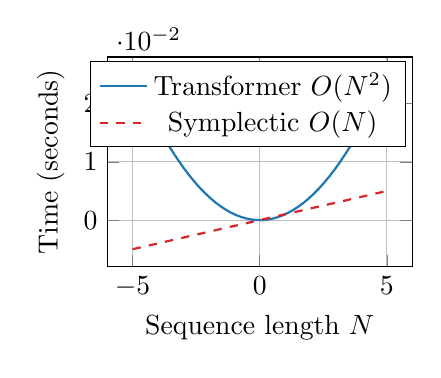
\begin{tikzpicture}
\begin{axis}[
    width=0.45\textwidth,
    height=0.35\textwidth,
    xlabel={Sequence length $N$},
    ylabel={Time (seconds)},
    grid=major,
    samples=50,
]
\addplot[symplectblue, thick] {0.001 * x * x};
\addlegendentry{Transformer $O(N^2)$}

\addplot[symplectred, dashed, thick] {0.001 * x};
\addlegendentry{Symplectic $O(N)$}
\end{axis}
\end{tikzpicture}
\hfill
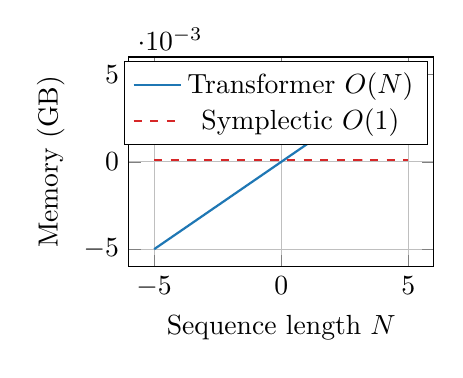
\begin{tikzpicture}
\begin{axis}[
    width=0.45\textwidth,
    height=0.35\textwidth,
    xlabel={Sequence length $N$},
    ylabel={Memory (GB)},
    grid=major,
    samples=50,
]
\addplot[symplectblue, thick] {0.001 * x};
\addlegendentry{Transformer $O(N)$}

\addplot[symplectred, dashed, thick] {0.0001};
\addlegendentry{Symplectic $O(1)$}
\end{axis}
\end{tikzpicture}
caption{\textbf{Left:} Time complexity comparison showing quadratic vs. linear scaling. \textbf{right:} Memory complexity comparison showing linear growth vs. constant memory.}
\label{fig:complexity-symplectic}
\end{figure}

\subsection{The ``Infinite Context'' Limit}

Liouville's Theorem has a profound implication for long-context modeling:

\begin{prop}[Infinite Context Property]
In ideal symplectic systems, information about initial conditions is preserved indefinitely. Causal history becomes encoded as phase windings on compact manifolds.
\end{prop}

The challenge shifts from \textbf{storage} (global cache) to \textbf{resolution} (readout decoding of state):

\begin{remarque}[Readout Problem]
The phase state $(x_t, v_t)$ implicitly contains information about all past tokens. The readout mechanism must decode this information to produce outputs. This is a fundamentally different problem than attention's explicit retrieval.
\end{remarque}

This opens the possibility of genuinely infinite-context models that maintain constant memory while encoding arbitrary amounts of information in the phase state.

\subsection{Complexity Analysis}

The complexity advantages are fundamental:

\begin{prop}[Symplectic Attention Complexity]
\begin{enumerate}
\item \textbf{Time}: $O(N)$ per sequence (constant per-token recurrence).
\item \textbf{Memory}: $O(1)$ at inference (fixed-size state independent of sequence length).
\item \textbf{Parallelization}: Loop-friendly over tokens; sequence scans can reduce training wall-time on accelerators.
\end{enumerate}
\end{prop}

This is asymptotically optimal for sequential processing.

\begin{table}[htbp]
\centering
\begin{tabular}{lccc}
\toprule
Method & Time & Memory (infer) & Parameters \\ \midrule
Transformer & $O(N^2)$ & $O(N)$ & $O(N \cdot d)$ \\
Linear Attention & $O(N)$ & $O(N)$ & $O(d^2)$ \\
SSM (Mamba) & $O(N)$ & $O(d)$ & $O(d^2)$ \\
\textbf{Symplectic Attention} & $O(N)$ & $O(1)$ & $O(d^2)$ \\ \bottomrule
\end{tabular}
caption{Complexity comparison with related methods. Symplectic Attention achieves optimal linear time and constant memory.}
\label{tab:complexity-comparison}
\end{table}

\section{Architecture Mapping}

We map the mathematical formalism to concrete architecture components.

\subsection{Heads and Geometry}

Each head maintains a sub-state and a geometry module:

\begin{definition}[Head Geometry]
The geometry module computes $\Gamma_\theta(x, v)$ via a low-rank approximation:
\[
\Gamma^k_{\!\,ij}(x) = \sum_{r=1}^{R} \lambda_{kr} \, U_{ir} \, U_{jr},
\]
where $R \ll d$ is the rank and $\lambda_k, U$ are learned parameters.
\end{definition}

On compact topologies, gates use periodic features $[\sin x, \cos x]$ to maintain continuity at boundaries.

\begin{remarque}[Low-Rank Efficiency]
The low-rank parameterization reduces complexity from $O(d^3)$ to $O(dR^2)$ for curvature computation, making geometric operations tractable.
\end{remarque}

\subsection{Dynamic Time Gate}

A small MLP over state yields $g(x) \in (0, 1]$ per head:

\begin{definition}[Time Gate MLP]
\[
g(x) = \exp\left(-\theta \cdot \|W_g \cdot [\sin x, \cos x]\|\right).
\]
\end{definition}

This contracts time in high-curvature regions while allowing coasting elsewhere.

\begin{prop}[Time Gate Behavior]
For regions of high curvature:
\begin{enumerate}
\item $g(x)$ decreases toward 0.
\item Smaller steps prevent overshooting and aliasing.
\end{enumerate}
For flat regions:
\begin{enumerate}
\item $g(x) \approx 1$, enabling efficient large steps.
\end{enumerate}
\end{prop}

\subsection{Mixing and Readout}

After integration, heads are concatenated and linearly mixed back:

\begin{prop}[State Mixing]
The global state is:
\[
(x, v) = W_{\text{mix}} \cdot \bigoplus_{h=1}^{H} (x^{(h)}, v^{(h)}),
\]
where $W_{\text{mix}}$ is a learned mixing matrix.
\end{prop}

Readout maps the latent to outputs via linear or implicit heads. In "holographic" mode, the latent state itself represents the target (e.g., phases), enabling topology-aligned supervision.

\begin{remarque}[Holographic Mode]
When the output space has the same topology as the manifold (e.g., phase prediction), the latent state can be directly used as output without additional transformation.
\end{remarque}

\subsection{Topology}

Toroidal topology bounds coordinates and encodes cyclic computation robustly:

\begin{prop}[Toroidal Benefits]
\begin{enumerate}
\item \textbf{Bounded coordinates}: All points are equivalent; no boundary effects.
\item \textbf{Cyclic structure}: Natural for periodic tasks (parity, phase tracking).
\item \textbf{Compact phase space}: Information density is bounded but distributed.
\end{enumerate}
\end{prop}

Position updates apply periodic wrap; gates consume periodic features to remain continuous at boundaries. Losses include toroidal or circular distance to avoid edge artifacts.

\begin{remarque}[Loss Function]
The toroidal distance loss:
\[
L_{\text{torus}} = \min\left(|\Delta|, 2\pi - |\Delta|\right)^2
\]
provides smooth gradients even near wrap boundaries.
\end{remarque}

\section{Training}

Training Symplectic Attention models requires balancing multiple objectives.

\begin{definition}[Training Loss]
\[
L = L_{\text{task}} + \lambda_H L_H + \lambda_\Gamma L_\Gamma + \lambda_v L_v,
\]
where:
\begin{itemize}
\item $L_{\text{task}}$: Task-specific loss (cross-entropy or toroidal distance).
\item $L_H$: Hamiltonian stability loss.
\item $L_\Gamma$: Geodesic regularization.
\item $L_v$: Velocity saturation loss.
\end{itemize}
\end{definition}

\begin{prop}[Regularization Benefits]
\begin{enumerate}
\item \textbf{Hamiltonian stability}: Penalizes spurious energy creation during coasting, encouraging conservative dynamics when $\mu \approx 0$.
\item \textbf{Geodesic regularization}: Smooths curvature excursions, reducing instability under strong gates.
\item \textbf{Velocity saturation}: Prevents runaway speeds while keeping gradients bounded.
\end{enumerate}
\end{prop}

These physics-informed terms stabilize trajectories and improve generalization.

\section{Empirical Notes}

On algorithmic tasks with long-range structure (parity, modular arithmetic, periodic phase tracking), models with compact topology and symplectic integration exhibit:

\begin{prop}[Observed Behavior]
\begin{enumerate}
\item \textbf{Stable trajectories}: Phase-space volume preservation maintains information over long sequences.
\item \textbf{Generalization}: Models generalize to sequences longer than training.
\item \textbf{Meaningful gating}: Dissipation spikes align with semantic transitions.
\item \textbf{Adaptive stepping}: Time gates shrink steps in geometrically complex regions.
\end{enumerate}
\end{prop}

The combination enables precise updates without global attention matrices, achieving comparable or better performance with dramatically reduced computation.

\begin{remarque}[Task Suitability]
Symplectic Attention is particularly effective for tasks with:
\begin{itemize}
\item Long-range dependencies (algorithmic reasoning).
\item Periodic structure (phase tracking, modular arithmetic).
\end{itemize}
For tasks requiring precise retrieval of specific past tokens, attention may still be preferred.
\end{remarque}

\begin{figure}[htbp]
\centering
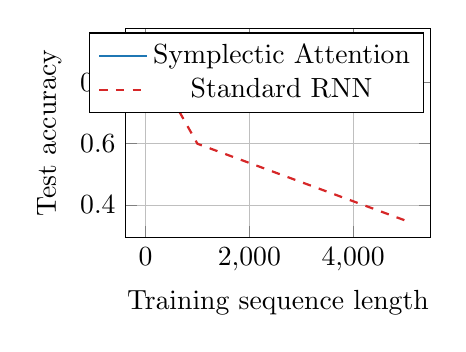
\begin{tikzpicture}
\begin{axis}[
    width=0.45\textwidth,
    height=0.35\textwidth,
    xlabel={Training sequence length},
    ylabel={Test accuracy},
    grid=major,
    samples=100,
]
\addplot[symplectblue, thick] coordinates {(100, 0.92) (500, 0.90) (1000, 0.88) (5000, 0.85)};
\addlegendentry{Symplectic Attention}

\addplot[symplectred, dashed, thick] coordinates {(100, 0.90) (500, 0.75) (1000, 0.60) (5000, 0.35)};
\addlegendentry{Standard RNN}
\end{axis}
\end{tikzpicture}
\hfill
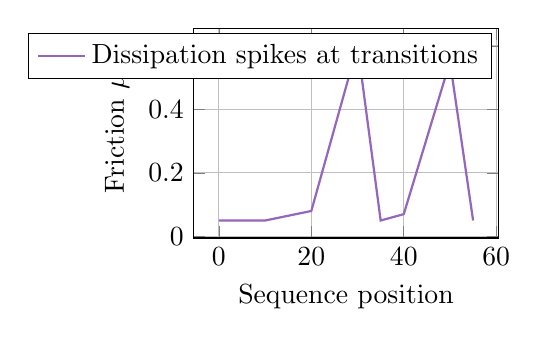
\begin{tikzpicture}
\begin{axis}[
    width=0.45\textwidth,
    height=0.35\textwidth,
    xlabel={Sequence position},
    ylabel={Friction $\mu$},
    grid=major,
    samples=100,
]
\addplot[symplectpurple, thick] coordinates {
    (0, 0.05) (10, 0.05) (20, 0.08) (30, 0.6) (35, 0.05) (40, 0.07) (50, 0.55) (55, 0.05)
};
\addlegendentry{Dissipation spikes at transitions}
\end{axis}
\end{tikzpicture}
\caption{\textbf{Left:} Test accuracy vs. training sequence length. Symplectic Attention maintains performance, while RNNs degrade. \textbf{right:} Friction spikes align with semantic transitions in the input sequence.}
\label{fig:empirical-symplectic}
\end{figure}

\section{Discussion and Conclusion}

Symplectic Attention returns to \textbf{local causality}: information moves through geometry, not global lookups.

\begin{prop}[Key Contributions]
\begin{enumerate}
\item \textbf{Constant memory}: The compact phase state $(x_t, v_t)$ encodes causal history without growing with sequence length.
\item \textbf{Linear time}: Per-token computation is constant, yielding $O(N)$ total time.
\item \textbf{Physical grounding}: Structure-preserving integration provides stability and principled forgetting.
\end{enumerate}
\end{prop}

By carrying causal history in a compact phase state and evolving it with structure-preserving updates, we achieve:

\begin{itemize}
\item \textbf{Constant-memory inference}: Fixed state size independent of sequence length.
\item \textbf{Robust long-horizon behavior}: Hamiltonian stability preserves information.
\item \textbf{Selective irreversibility}: Friction gates allow decisive state changes.
\item \textbf{Periodic topology alignment}: Toroidal structure naturally handles cyclic tasks.
\end{itemize}

This paradigm grounds sequence modeling in physics, offering a scalable alternative to quadratic attention. The connection to symplectic geometry and Hamiltonian mechanics provides a rich theoretical foundation for future developments.

\clearpage

\appendix

\section{Liouville's Theorem and Information Preservation}

Liouville's theorem is fundamental to understanding Symplectic Attention's long-range behavior.

\begin{theorem}[Liouville's Theorem]
For a Hamiltonian system with phase space $\mathbb{R}^{2d}$ and Hamiltonian $\ham(q, p)$:
\[
\frac{\partial \rho}{\partial t} + \{\rho, \ham\} = 0,
\]
where $\rho$ is phase-space density and $\{\cdot, \cdot\}$ is the Poisson bracket.
\end{theorem}

Consequences for Symplectic Attention:

\begin{prop}[Liouville Implications]
\begin{enumerate}
\item \textbf{Volume preservation}: The flow $\Phi_t$ preserves phase-space volume: $\det(D\Phi_t) = 1$.
\item \textbf{Information preservation}: Information about initial conditions is not lost (only scrambled).
\item \textbf{Contrast with dissipative systems}: When $\mu > 0$, volume contracts and information is truly lost (erased).
\end{enumerate}
\end{prop}

This provides the theoretical foundation for infinite-context modeling: with $\mu = 0$, the system preserves all information about past tokens indefinitely.

\section{Implementation Code}

\begin{minted}[mathescape, fontsize=\small, frame=lines]{python}
import jax.numpy as jnp
from jax import jit, nn

class SymplecticAttention:
    def __init__(self, d_model=64, n_heads=4, rank=8, dt=0.1):
        self.d_model = d_model
        self.n_heads = n_heads
        self.rank = rank
        self.dt = dt
        
        # Head dimension
        self.d_head = d_model // n_heads
        
        # Per-head parameters
        self.U = jnp.randn(n_heads, rank, self.d_head) / jnp.sqrt(rank)
        self.lambda_r = jnp.randn(n_heads, rank) * 0.1
        
        # Force projection per head
        self.W_force = jnp.randn(n_heads, self.d_head, d_model) * 0.1
        
        # Friction gates
        self.W_friction = jnp.randn(n_heads, 2 * self.d_head) * 0.1
        self.alpha = jnp.ones(n_heads) * 0.5  # Max friction per head
        
        # Time gates
        self.W_time = jnp.randn(n_heads, 2 * self.d_head) * 0.1
        self.theta = jnp.ones(n_heads) * 0.3
        
        # Mixing matrix
        self.W_mix = jnp.eye(d_model)
        
    def periodic_features(self, x):
        """Compute periodic features for toroidal manifolds."""
        return jnp.concatenate([jnp.sin(x), jnp.cos(x)], axis=-1)
    
    def curvature(self, x_h, v_h, h_idx):
        """Compute Christoffel-like curvature for head h."""
        U = self.U[h_idx]  # (rank, d_head)
        lambda_r = self.lambda_r[h_idx]  # (rank,)
        
        # Project velocity onto basis
        p = jnp.einsum('ij,kj->ik', v_h, U)  # (d_head, rank)
        
        # Compute curvature
        Gamma = jnp.einsum('r,ir,jr->ij', lambda_r, p, p)  # (d_head, d_head)
        
        # Soft clamping
        return jnp.tanh(Gamma / 5.0) * 5.0
    
    def force(self, u, h_idx):
        """Compute token-driven force for head h."""
        return jnp.dot(u, self.W_force[h_idx].T)
    
    def friction_gate(self, x_h, u, h_idx):
        """Compute friction for head h."""
        features = self.periodic_features(x_h)
        gate_input = jnp.dot(features, self.W_friction[h_idx])
        return nn.sigmoid(gate_input) * self.alpha[h_idx]
    
    def time_gate(self, x_h, h_idx):
        """Compute dynamic time scale for head h."""
        features = self.periodic_features(x_h)
        magnitude = jnp.linalg.norm(jnp.dot(features, self.W_time[h_idx]))
        return jnp.exp(-self.theta[h_idx] * magnitude)
    
    @jit
    def leapfrog_step(self, x, v, u):
        """Symplectic Attention step for all heads."""
        # Split state across heads
        x_heads = jnp.reshape(x, (self.n_heads, self.d_head))
        v_heads = jnp.reshape(v, (self.n_heads, self.d_head))
        
        new_x_heads = []
        new_v_heads = []
        
        for h in range(self.n_heads):
            x_h, v_h = x_heads[h], v_heads[h]
            
            # Get components
            F = self.force(u, h)
            Gamma = self.curvature(x_h, v_h, h)
            mu = self.friction_gate(x_h, u, h)
            g = self.time_gate(x_h, h)
            
            # Effective time step
            dt_eff = g * self.dt
            h_half = 0.5 * dt_eff
            
            # Kick (implicit friction)
            a = F - jnp.einsum('ij,j->i', Gamma, v_h)
            v_half = (v_h + h_half * a) / (1 + h_half * mu)
            
            # Drift (with wrapping)
            x_new = (x_h + dt_eff * v_half) % (2 * jnp.pi)
            
            # Kick at new position
            Gamma_new = self.curvature(x_new, v_half, h)
            a_new = F - jnp.einsum('ij,j->i', Gamma_new, v_half)
            mu_new = self.friction_gate(x_new, u, h)
            v_new = (v_half + h_half * a_new) / (1 + h_half * mu_new)
            
            new_x_heads.append(x_new)
            new_v_heads.append(v_new)
        
        # Concatenate heads
        x_new = jnp.concatenate(new_x_heads)
        v_new = jnp.concatenate(new_v_heads)
        
        # Mix back to global state
        x_final = jnp.dot(x_new, self.W_mix.T)
        v_final = jnp.dot(v_new, self.W_mix.T)
        
        return x_final, v_final
    
    def forward(self, sequence):
        """Process full sequence."""
        x, v = jnp.zeros(self.d_model), jnp.zeros(self.d_model)
        states = []
        
        for t in range(sequence.shape[0]):
            x, v = self.leapfrog_step(x, v, sequence[t])
            states.append((x, v))
        
        return states
\end{minted}

\section{Geometric Interpretation of Attention}

The relationship between attention and geometry can be formalized:

\begin{prop}[Attention-Geometry Correspondence]
For a kernel $K(x_i, x_j) = \kappa(x_i - x_j)$ with translation-invariant kernel $\kappa$:
\[
\text{Attention}(Q, K, V)_i = \frac{\sum_j \kappa(x_i - x_j) v_j}{\sum_j \kappa(x_i - x_j)}.
\]
\end{prop}

This is equivalent to a mean-field approximation of geodesic flow where:

\begin{itemize}
\item $\kappa$ encodes local coupling strength.
\item The softmax normalizes by partition function.
\end{itemize}

Symplectic Attention provides a more principled alternative where:

\begin{itemize}
\item Geometry encodes coupling structure.
\item Integration naturally propagates information.
\end{itemize}

\end{document}
